\documentclass[12pt]{article}

\usepackage{sbc-template}

\usepackage{graphicx,url}

\usepackage[brazil]{babel}   
\usepackage[utf8]{inputenc}  

     
\sloppy

\title{Resolução de um Problema de Otimização utilizando \\o Algoritmo Ant System}

\author{Diego Rubin\inst{1}}


\address{Departamento de Matemática Aplicada e Computação \\
  - Universidade Estadual Paulista "Julio de Mesquita Filho"
  (UNESP)\\
  Rio Claro -- SP -- Brazil
  \email{rubin.diego@gmail.com}
}

\begin{document} 

\maketitle

\begin{abstract}
This article aims desmotrar the concepts presented 
during the course Evolutionary Computing, taught 
by PhD Adriane Beatriz Serapião, showing 
the results achieved in the implementation of the 
Ant System algorithm for solving an optimization problem.
\end{abstract}

\begin{resumo} 
Este artigo tem como objetivo desmotrar
os conceitos apresentados durante a 
disciplina Computação Evolutiva, ministrada
pela Profa. Dra. Adriane Beatriz Serapião,
mostrando os resultados obtidos na implementação
do algoritmo Ant System para resolução de um
problema de otimização.
\end{resumo}


\section{Introdução}

Problemas de otimização são frequentes no nosso coditiano e exitem 
diversas formas de encontrarmos soluções para os mesmos. Neste artigo
será apresentado um exemplo de solução para um problema de otimização
utilizando um algoritmo chamado Ant System proposto por M. Dorigo e V. Maniezzo
\cite{AS}.

O algoritmo foi implementado em uma linguagem chamada Python e o 
código gerado pelo ser encontrado em http://github.com/diegorubin/Evolutionary-Computation/tree/master/final/src.

A linguagem Python foi escolhida para a implementação do 
algoritmo por causa da facilidade de trabalho com listas e 
iterações. Além disso abstrai problemas que podiamos ter
em outras linguagens, como por exemplo C e Pascal, quando
memória precisa ser alocadas para utilizarmos vertores
e matrizes.

\section{O Problema} \label{sec:firstpage}

O Problema que será abordado com fins de demonstração do algoritmo
foi proposto pelo Prof. Eduardo C. Xavier do IC da Unicamp e pode
ser encontrado em \cite{xavier}. 
O enunciado do problema diz:

Você possui uma empresa reconhecida na área de otimização e algoritmos. 
Um dia e chamado por telefone para uma conversa urgente com um grupo 
de pessoas que está trabalhando em um grande projeto: “Salvar o mundo”. 
Eles lhe informam que trabalham para um ministério da ONU sob 
supervisão de vários países.

Devido a dificuldade para se estabelecer um acordo sobre metas de 
redução de emissção de carbono por parte dos países, este grupo deve 
achar uma outra solução para o problema do aquecimento global. 

Este grupo e formado por cientistas e engenheiros, que desenvolveram
uma solucao (não muito boa mas a melhor possível): Emitir dióxido 
de enxofre na estratosfera, pois este gás reflete grande parte dos 
raios solares e funcionaria como um filtro solar para a Terra, 
invertendo a trajetória de aumento de temperatura. A idéia é construir 
torres com canos enormes que levariam o dióxido de enxofre até a estratosfera. 
Estes são chamados de sistemas de emissão. Dependendo do lugar onde 
este gás é liberado, ele cobrirá diferentes partes do céu, devido as 
correntes de ar existentes. Dado uma posição para instalação do sistema 
de emissão, e dado as correntes de ar existentes, pode-se prever com 
certa precisão quais lugares da Terra será coberto por esta camada 
“protetora”. Para a instalação de um sistema de emissão, há um custo 
monetário e ecológico que varia dependendo do lugar onde este é instalado. 
O objetivo e determinar os lugares de instalação dos sistemas de emissão 
de tal forma que toda a Terra seja coberta pelo dióxido de enxofre, e ao 
mesmo tempo se minimize o custo de instalação dos sistemas de emissão. 
O espaço contínuo a ser coberto (a superfície da Terra) será discretizado, 
de tal forma que temos pontos que devem ser cobertos, como ilustrado
na Figura 1. 

\begin{figure}
\centering
\includegraphics[width=.8\textwidth]{pontos.ps}
\caption{(a) Exemplo da Terra com superfície discretizada (b) Pontos 
cobertos por um sistema de emissão (c)Pontos cobertos por um segundo sistema de emissão.}
\end{figure}

\section{Metodologias}

O algortimo que iremos utilizar para obter um bom resultado para o problema
descrito é um algoritmo do tipo Ant Colony Optimization(ACO) chamado Ant System.
Ele foi proposto por M. Dorigo e V. Maniezzo e é muito utilizado em 
problemas onde o objetivo é encontrar o rotas.

Algumas adaptações serão feitas para podemos utilizar este algoritmo para
resolvermos o problema. O nosso objetivo é encontrar o menor custo para 
construirmos as torres para cobrir todos os pontos. A principio utilizaremos
o custo de cada torre em substituição a distâncias que comumente é utilizado no problemas
onde o algoritmo é aplicado. Porém somente esta substituição não irá
colaborar muito para encontrarmos um valor bom ou ótimo para a função 
objetivo, pois as distâncias entre as torres serão iguais entre si. Outra
adaptação que será utilizada será baseada no fato que as torres podem
cobrir pontos iguais, então iremos alterar a heurística utilizada para calcular
as distâncias entre as torres utilizando o fator obtido pelos pontos iguais que são 
cobertos entre as torres. Por exemplo, se a torre S1 cobrir as pontos 1, 2 e 3 e 
e a torre S2 cobrir os pontos 2, 3 e 4 a distancia entre as duas torres
será dada por $((a+b)/2)*(c+1)$ onde $a$ e $b$ são os custos de construção de 
cada torre e $c$ o número de pontos cobertos em comum. Esta medida é tomada
para que não seja utilizada somente o custo como base de escolha e acabe escolhendo
torres que cobrem pontos já cobertos.

O ponto de parada escolhido nos testes foram o número de iterações. Após
100 iterações o programa é encerrado.

\section{Atualização dos Ferômonios}

Uma das fases mais importantes do algoritmo Ant System é a Atualização
de Ferormonios. Enquanto as formigas caminham elas liberar hormonios que funcionam
como uma espécie de guia para outras formigas se não houver um uma disperção do hormonio
as formigas podem tender a um caminho que não é o bom ou ótimo. A regra de atualização
é dada por $(1-p)\tau_{ij} + \sum_{k=1}^{m}\delta\tau_{ij}^{(k)}$. Após gerar uma
solução, ou seja, após todas formigas chegarem ao seu destino a matriz com 
o valor do depósito em cada aresta é atualizado utilizando a regra descrita anteriormente.

\section{Entrada dos Dados}

O programa criado tem como entrada de dados um arquivo texto que deve estar no mesmo
diretório em que a aplicação será executada e deve possuir o nome "entrada".

O arquivo de entrada deve conter na primeira linha o número de pontos que devem ser cobertos pelas torres e
as linhas seguintes devem conter o nome da torre, o seu custo e os pontos que
são cobertos por ela. Um arquivo que não estiver formatado desta forma poderar
gerar erros, assim não chegando a um resultado válido ou o término prematuro da
aplicação.

\section{Parâmetros do Algoritmo}

O algoritmo permite a variação de alguns parâmetros para melhor obtenção do resultados.
Um deles é a relação probabilistica entre os fatores heuristicos ou os hormonios depositados
pelas formigas, $\alpha$ e $\beta$. Esta relação é importante para que as formigas não fiquem
muito dependentes dos hormonios ou da decisão local de qual caminho seguir baseado
apenas na menor distancia.

Outro parametro importante é o fator de evaporação dos hormonios $p$, que foi apresentado na 
equação de Atualização do Ferômonios, que também servepara que o algoritmo não entre 
em estagnação muito rápido.

A única forma para esolhermos quais são os melhores parâmetros a serem escolhidos
é testarmos nossa aplicação e compararmos resultados.

\section{Resultados}
Para fins de estudo, um gerador de dados para a entrada será utilizado. Este
gerador pode ser obtido no mesmo endereço onde o problema está localizado.

O caso de testes que será apresentado possui 20 pontos a serem cobertos
pelas antenas, essa entrada pode ser vista na Tabela 1. A Tabela 2 exibe os resultados 
dos testes realizados com esses dados.

\begin{table}

\centering

\caption{Dados de entrada do Primeiro Caso de Teste}
\begin{tabular}{cccc}

\hline
Nome da Torre & Custo & Pontos Cobertos\\

\hline
\hline

S1 & 9.95301754277 & 4 7 8 \\
S2 & 15.758625561 & 2 3 4 5 9 10 11 16 \\
S3 & 23.4868725572 & 4 8 14 20 \\
S4 & 23.0675439215 & 2 7 11 12 13 14 16 19 \\
S5 & 13.3142020168 & 3 7 9 10 13 14 15 \\
S6 & 12.2247929853 & 7 15 17 19 \\
S7 & 13.3551096088 & 1 4 18 \\
S8 & 10.2618923987 & 1 9 11 12 18 \\
S9 & 9.52730129955 & 9 12 \\
S10 & 23.9058218015 & 10 16 17 \\
S11 & 8.70159012372 & 6 \\
S12 & 10.4651515915 & 11 13 15 17 19 \\
S13 & 14.2921462405 & 7 11 \\
S14 & 6.81050785913 & 6 17 20 \\
S15 & 8.59062534436 & 3 5 6 16 \\
S16 & 12.3151153804 & 5 10 11 13 \\
S17 & 15.8773771887 & 1 2 3 5 7 9 10 \\
S18 & 9.44317635859 & 1 2 3 8 10 12 17 19 20 \\
S19 & 6.60212341378 & 1 2 7 8 9 13 17 20 \\
S20 & 8.41965820277 & 2 3 8 9 13 15 \\
S21 & 23.2571733263 & 6 \\
S22 & 10.6192126916 & 4 5 6 9 10 13 15 17 19 20 \\
S23 & 7.96498144685 & 4 5 6 8 9 10 11 15 17 18 \\
S24 & 19.4505655714 & 11 17 19 \\
S25 & 19.3232534171 & 9 16 18 19 20 \\
S26 & 19.5909681765 & 2 4 5 8 10 13 16 \\
S27 & 15.209911175 & 6 9 10 18 \\
S28 & 24.163810892 & 2 15 16 \\
S29 & 10.0755402387 & 3 6 7 10 12 19 \\
S30 & 21.5523554772 & 8 9 11 15 17 20 \\
S31 & 19.4291897147 & 1 5 6 9 10 13 14 16 \\

\hline
\end{tabular}
\label{tab1}
\end{table}



\begin{table}

\centering

\caption{Resultados obtidos}
\begin{tabular}{cccc}

\hline
$\alpha$ & $\beta$ & $p$ & Valor Recorrente(Aproximado)\\

\hline
\hline

1 & 2 & 0.2 & 47 \\
1 & 1 & 0.2 & 40 \\
2 & 1 & 0.2 & 52 \\
1 & 2 & 0.5 & 48 \\
1 & 1 & 0.5 & 40 \\
2 & 1 & 0.5 & 40 \\
1 & 2 & 0.8 & 40 \\
1 & 1 & 0.8 & 47 \\
2 & 1 & 0.8 & 40 \\

\hline
\end{tabular}
\label{tab2}
\end{table}

Foi possível notar que com os parâmetros $\alpha=1$, $\beta=2$ e $p=0.8$ a estagnação
acontece mais lentamente e o resultado, na maioria das vezes, acaba convergindo
para um bom resultado. Isso acontece porque o ferômonio evapora mais rápido e novos
caminhos podem ser explorados pelas formigas.
Diferente do que acontece com os parâmetros $\alpha=2$, $\beta=1$ e $p=0.2$ onde a 
estagnação acontece rápidamente, e muitas das vezes um valor com não é obtido.
Os valores obtidos que estão na tabela os valores mais frequentes dentre
10 execuções da aplicação.

\section{Conclusão}

De acordo com os resultados obtidos, é possível notar que
o Ant System consegue sempre encontrar um valor bom para 
a função objetivo, porém muitas vezes ele acaba não encontrando 
o valor ótimo.

A aplicação foi testada com diversas entradas variando os números de pontos 
a serem cobertos e torres à serem analisadas e pode-se perceber que
para números de torres maiores que 250 a aplicação começa a demorar muito
para obter uma solução.

Há diversas otimizações que poderiam ser feitas no código da aplicação
para que a mesma pudesse abranger um número maior de casos mais rápidamente,
porém nosso objetivo era mostrar um exemplo de como o algoritmo funciona e 
como ele pode ser aplicado e este objetivo foi alcançado.

\bibliographystyle{sbc}
\bibliography{relatorio}

\end{document}
